\documentclass[aspectratio=169,11pt]{beamer}
% Shared preamble for the CogLean decks.
% Build the slides alone, or with speaker notes (see the Makefile):
%   pdflatex deck.tex                                   -> slides
%   pdflatex -jobname=deck-notes "\def\withnotes{}\input{deck.tex}"  -> slides + notes
\usetheme{default}
\usecolortheme{seahorse}
\setbeamertemplate{navigation symbols}{}
\setbeamertemplate{footline}[frame number]
\setbeamerfont{note page}{size=\small}
\setbeamercolor{note page}{bg=white}
\ifdefined\withnotes
  \setbeameroption{show notes}
\fi
\usepackage[T1]{fontenc}
\usepackage{lmodern}
\usepackage{booktabs}
\usepackage{amsmath,amssymb}
\usepackage{tikz}
\usetikzlibrary{positioning,arrows.meta,shapes.misc}
\tikzset{
  box/.style={draw, rounded corners, align=center, minimum height=8mm, inner sep=4pt, fill=blue!6},
  arr/.style={-{Stealth[length=2mm]}, thick}
}
\newcommand{\code}[1]{\texttt{#1}}
\newcommand{\has}{\textbf{has}}
\newcommand{\lacks}{\textcolor{red!70!black}{lacks}}
\newcommand{\never}{\textcolor{red!70!black}{\textbf{never}}}
\newcommand{\canhold}{can hold}

% Lean source in slides: fvextra Verbatim, with the Unicode Lean uses mapped
% to math symbols (pdflatex).
\usepackage{fvextra}
\fvset{fontsize=\scriptsize, frame=single, framesep=2mm, rulecolor=\color{gray!50},
  breaklines=true, breakanywhere=false}
\DeclareUnicodeCharacter{2192}{\ensuremath{\to}}
\DeclareUnicodeCharacter{2190}{\ensuremath{\leftarrow}}
\DeclareUnicodeCharacter{2194}{\ensuremath{\leftrightarrow}}
\DeclareUnicodeCharacter{2200}{\ensuremath{\forall}}
\DeclareUnicodeCharacter{2203}{\ensuremath{\exists}}
\DeclareUnicodeCharacter{27E8}{\ensuremath{\langle}}
\DeclareUnicodeCharacter{27E9}{\ensuremath{\rangle}}
\DeclareUnicodeCharacter{2260}{\ensuremath{\neq}}
\DeclareUnicodeCharacter{2227}{\ensuremath{\wedge}}
\DeclareUnicodeCharacter{2228}{\ensuremath{\vee}}
\DeclareUnicodeCharacter{00AC}{\ensuremath{\neg}}
\DeclareUnicodeCharacter{2264}{\ensuremath{\le}}
\DeclareUnicodeCharacter{2208}{\ensuremath{\in}}
\DeclareUnicodeCharacter{2209}{\ensuremath{\notin}}
\DeclareUnicodeCharacter{00D7}{\ensuremath{\times}}
\DeclareUnicodeCharacter{03B1}{\ensuremath{\alpha}}
\DeclareUnicodeCharacter{03B2}{\ensuremath{\beta}}
\DeclareUnicodeCharacter{03BC}{\ensuremath{\mu}}
\DeclareUnicodeCharacter{03B8}{\ensuremath{\theta}}
\DeclareUnicodeCharacter{2218}{\ensuremath{\circ}}
\DeclareUnicodeCharacter{25B8}{\ensuremath{\blacktriangleright}}
\DeclareUnicodeCharacter{00B7}{\ensuremath{\cdot}}
\DeclareUnicodeCharacter{2026}{\ldots}

\usepackage{array}
\tikzset{src/.style={rounded corners=8pt, draw=none, align=center, inner sep=6pt,
    text width=#1, font=\small\bfseries, execute at begin node={\hyphenpenalty=10000\exhyphenpenalty=10000}},
  src/.default=3.5cm,
  to/.style={-{Stealth[length=2.2mm]}, thick, black!80}}

\title{CogLean}
\subtitle{Towards a Cumulative, Machine-Checked Theory of Cognition}
\author{Jeff Shrager}
\date{November 2026\\[2mm]\small\textcolor{red!70!black}{\textbf{Draft for Comment}}}

\begin{document}

% Head slides: the word, then where it came from.
\begin{frame}[plain]
  \begin{tikzpicture}[remember picture,overlay]
    \node at (current page.center) {\fontsize{54}{60}\selectfont\bfseries\itshape Epoofany};
  \end{tikzpicture}
\end{frame}
\note{
Epoofany.
}

\begin{frame}[plain]
  \begin{tikzpicture}[remember picture,overlay]
    \node[draw=orange!80!black, very thick, rounded corners=10pt, fill=orange!8,
          align=center, inner sep=8pt] (c) at (current page.center)
      {{\fontsize{40}{46}\selectfont\bfseries CogLean}\\[-2pt]
       \rule{4.2cm}{0.6pt}\\[2pt]
       {\itshape Don't just run models,}\\ {\itshape reason about them.}};
    \begin{scope}[shift={(current page.center)}]
      \node[src=3.7cm, fill=blue!12] (tl) at (-5.2, 2.85)
        {Reanimation of Simon \& Newell's early AIs\\ {\mdseries\itshape (esp.\ LT and EPAM)}};
      \node[src=3.3cm, fill=violet!12] (tc) at (0, 3.1)
        {Discussion with Pete and Chris on models of scientific reasoning};
      \node[src=3.6cm, fill=violet!18] (tr) at (5.2, 2.85)
        {NSS's theory of computer programs as cognitive models};
      \node[src=3.4cm, fill=green!12, align=left] (ml) at (-5.9, 0)
        {Training with Simon and Klahr during the {\mdseries\itshape Scientific Cognition} period};
      \node[src=3.4cm, fill=yellow!18] (mr) at (5.9, 0)
        {Work with Siegler on the DOA model};
      \node[src=3.4cm, fill=red!12] (bl) at (-5.2, -2.9)
        {Work with Anderson on ACT};
      \node[src=3.4cm, fill=blue!12] (br) at (5.2, -2.9)
        {The Lean-driven mathpocalypse};
    \end{scope}
    \draw[to] ([yshift=-2mm]tl.east) -- ([xshift=4mm]c.north west);
    \draw[to] (tc.south) -- (c.north);
    \draw[to] ([yshift=-2mm]tr.west) -- ([xshift=-4mm]c.north east);
    \draw[to] (ml.east) -- (c.west);
    \draw[to] (mr.west) -- (c.east);
    \draw[to] ([yshift=2mm]bl.east) -- ([xshift=4mm]c.south west);
    \draw[to] ([yshift=2mm]br.west) -- ([xshift=-4mm]c.south east);
  \end{tikzpicture}
\end{frame}
\note{
Where CogLean came from.
}

\begin{frame}
  \titlepage
\end{frame}
\note{
This talk goes with the paper of the same name, which is a draft for comment. It hasn't been carefully checked yet: think of it as an over-starched blog post, and constructive feedback is welcome. It introduces CogLean, a library of cognitive theory in the Lean proof assistant, and argues for a way of doing theoretical cognitive science: theories stated once, their consequences proved, and results that accumulate, compose and transfer. I'm going to tell it partly through a hypothetical modeler, Chris, who uses the library to answer two questions: one forward, from a phenomenon to a theorem, and one backward, from a proposed regularity to what a theory must be like to produce it. Companion talks and papers take it further, to a model of multi-digit addition and to concept formation. And one thing up front: this is less about proof, in the usual sense, than about explanation. The theorems are explanations of phenomena, and Lean keeps them aligned with the programs they explain.
}
\begin{frame}{The problem: making theory cumulative}
  \begin{itemize}
    \item Newell (1973): twenty questions with nature, answers never assembled; Newell (1990): unified theories.
    \item Cognitive architectures (Soar, ACT-R; now the Common Model) have spent decades on this: \textbf{shared mechanisms}, so models of different tasks reuse and integrate theoretical commitments.
    \item What they accumulate is mainly \textbf{models}: what a model predicts is established by running it, one setting at a time, and a result for one model is rarely reusable \emph{as a result} by another.
    \item CogLean, \textbf{complementary}: accumulate machine-checked \textbf{theorems} about mechanisms, reusable deductively, and stated across architectural commitments.
  \end{itemize}
  \bigskip
  \emph{Can cognitive theory be organized the way Mathlib organizes mathematics: definitions made once, results proved, and later work building on earlier results?}
\end{frame}
\note{
The problem is an old one, and the people who have done the most about it are the architecture builders. Newell complained in 1973 that we play twenty questions with nature and never assemble the answers, and his answer was unified theories of cognition. Soar and ACT-R, and now the Common Model of Cognition, are decades of work by Newell, Anderson, Laird, Rosenbloom and many others on exactly this: shared mechanisms and constraints, so that a model of a new task reuses the architecture's theory of memory, learning and control, and models of different tasks can be integrated. CogLean is not the first effort in this direction, and it isn't a competitor. What architectures accumulate, though, is mainly models. What a model predicts is established by running it, at one setting at a time, and a result established for one model is rarely available as a result to another. CogLean pursues a complementary goal: accumulating machine-checked theorems about cognitive mechanisms, which can be reused deductively, and stated independently of any one architecture's commitments, so they can cover classes of mechanisms. An architecture could, in principle, carry such results itself. The question for this talk is whether cognitive theory can be organized the way mathematics has been organized in Mathlib, so that results, and not only models, accumulate.
}

\begin{frame}{Formalizing explanations}
  \begin{itemize}
    \item \textbf{Phenomena}: regularities of behavior, stated without any mechanism. Observed, they are \textbf{psychological facts}; derived but not yet observed, they are \textbf{predictions}.
    \item \textbf{Mechanisms and assumptions}: postulates, conditions, laws.
    \item \textbf{Explanations}: deductions of a phenomenon from mechanisms and assumptions (a theorem and its lemmas).
    \item \textbf{Deduction}: what Lean checks. Given these mechanisms and assumptions, the phenomenon follows; whether they hold of people is for experiments.
  \end{itemize}
  \medskip
  The explanation is a proof about \textbf{the same program that runs}: change the model, and every explanation it breaks fails to check.
  \medskip

  \small A phenomenon can have several explanations; a mechanism can help explain several phenomena.
\end{frame}
\note{
Before any Lean, here's what this is for. It's less about proof, in the usual sense, than about explanation. What we explain are phenomena, stated without any mechanism: observed, they're psychological facts; derived but not yet observed, they're predictions. Underneath are mechanisms and their assumptions: postulates, conditions and laws. An explanation is a deduction of a phenomenon from those, in Lean a theorem and its chain of lemmas. That's Hempel and Oppenheim's old deductive picture of explanation, running through how the mechanisms work, made checkable. Lean proves conditional statements; whether the assumptions hold of people is for experiments. And here's what I think matters most. Usually a model is a program and its explanation lives somewhere else, in prose or in math about an idealized program, and the two drift apart. In Lean, the definitions that run are the ones the theorems are about, so when the model changes, every explanation it breaks fails to check, and the rest are confirmed. Not every proof is an explanation; that stays a judgment. But one phenomenon can have several explanations, and one mechanism can help explain several phenomena, and a library of them lets us ask what observations would tell explanations apart.
}

\begin{frame}{Prior formal approaches to cognitive theory}
  \scriptsize
  \begin{tabular}{>{\raggedright\arraybackslash}p{0.34\linewidth}>{\raggedright\arraybackslash}p{0.19\linewidth}>{\raggedright\arraybackslash}p{0.36\linewidth}}
    \toprule
    Work & Formalism & What it establishes\\
    \midrule
    Soar specified in Z (Milnes et al.\ 1992) & Z notation & a complete, low-level, non-executable specification of one architecture\\
    Sceptic (Cooper, Fox, Farringdon \& Shallice 1996) & executable specification language & models (Soar among them) stated in a language designed for cognitive models\\
    Reconstructing ACT-R (Stewart \& West 2007) & Python reimplementation & core commitments separated from implementation; alternative components\\
    ACT-R operational semantics (Gall \& Fr\"uhwirth 2018) & abstract semantics; CHR & a translation proved sound and complete; confluence tests\\
    ACT-R as timed automata (Langenfeld et al.\ 2019, 2021) & timed automata & exhaustive defect analysis of models; the semantics proved correct\\
    A common formal ground for architectures (Ragni et al.\ 2018) & formal framework & ACT-R and Soar embedded for comparison\\
    Soar to PRISM (Ganeriwala et al.\ 2026) & Markov chains, PRISM & probabilistic model checking of stochastic models\\
    Verbal theories as logic programs; as automata (Rohner \& Kjellerstrand 2021; Finkel et al.\ 2025) & Prolog; automata & what a verbal theory's premises entail\\
    Critical tests from core assumptions (Fisher et al.\ 2025) & proofs in prose over model classes & which processing structures ACT-R's core rules out\\
    \bottomrule
  \end{tabular}
\end{frame}
\note{
CogLean is far from the first formal treatment of cognitive theory, and it's worth seeing what came before. In 1992 Milnes and colleagues specified Soar in the Z notation: complete, but low-level and not executable. Cooper, Fox, Farringdon and Shallice argued in 1996 for languages designed for specifying cognitive models, and built one, Sceptic. Stewart and West rebuilt ACT-R to separate its core commitments from its implementation. For ACT-R there's a formal operational semantics with a translation proved sound and complete, and a line of work translating ACT-R models into timed automata for exhaustive defect checking. Ragni and colleagues proposed a common formal ground into which ACT-R and Soar can be embedded. Most recently, Soar models have been compiled for the PRISM probabilistic model checker. Outside architectures, verbal theories have been formalized as logic programs and as automata, and Fisher and colleagues derived critical tests of ACT-R from its core assumptions. Almost all of this work formalizes one architecture or one model at a time, and establishes properties of that system. That's the contrast I'll come back to.
}

\begin{frame}{The analogy: Mathlib}
  \begin{itemize}
    \item Mathlib, the community library of formalized mathematics in Lean, proposes no new mathematics.
    \item It is a \textbf{shared environment}: definitions made once, every result machine-checked, later work citing earlier results.
    \item A theorem about groups, once proved, is available to everyone who uses groups.
  \end{itemize}
  \bigskip
  CogLean asks whether cognitive theory can be organized the same way.\\
  It is not a new theory of cognition, nor a new modeling language.\\
  And it is nowhere near Mathlib's scale: a first demonstration.
\end{frame}
\note{
Mathematics faced a version of this problem and has made real progress on it. Mathlib, the community library for the Lean proof assistant, doesn't propose new mathematics. It's a shared environment: definitions are made once, every result is checked by machine, and later work builds on earlier results by citing them. A theorem about groups, once proved, is available to everyone who works with groups. CogLean asks whether cognitive theory can be organized the same way. It is not a new theory of cognition, and it's not a new modelling language either. And it's nowhere near Mathlib's scale; this is a first demonstration that the approach can work.
}

\begin{frame}{CogLean's layers}
  \begin{center}
  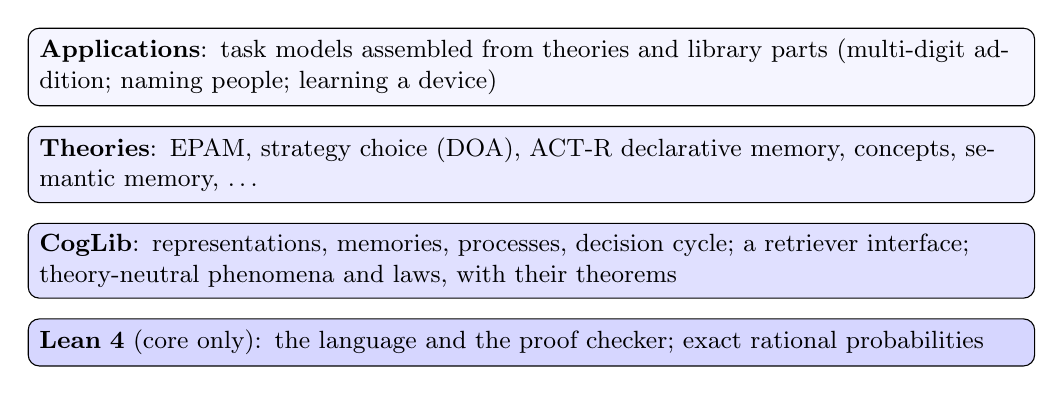
\begin{tikzpicture}[font=\small, node distance=2.5mm,
    layer/.style={draw, rounded corners, text width=12.5cm, align=left, inner sep=4pt}]
    \node[layer, fill=blue!4] (app) {\textbf{Applications}: task models assembled from theories and library parts (multi-digit addition; naming people; learning a device)};
    \node[layer, fill=blue!8, below=of app] (th) {\textbf{Theories}: EPAM, strategy choice (DOA), ACT-R declarative memory, concepts, semantic memory, \dots};
    \node[layer, fill=blue!12, below=of th] (lib) {\textbf{CogLib}: representations, memories, processes, decision cycle; a retriever interface; theory-neutral phenomena and laws, with their theorems};
    \node[layer, fill=blue!16, below=of lib] (lean) {\textbf{Lean 4} (core only): the language and the proof checker; exact rational probabilities};
  \end{tikzpicture}
  \end{center}
  Each layer imports only those below it, and inherits their theorems.
\end{frame}
\note{
CogLean has four layers. At the bottom is Lean, core only, with exact rational probabilities. Above it is CogLib, the general library: representations such as feature codes and distributions; memory structures such as discrimination nets and an activation memory; processes such as sampled retrieval and a decision cycle with impasses; an interface that any memory can implement; and theory-neutral statements of phenomena and laws, with theorems about them. Above that are the theories, each stated as choices of library mechanisms. And at the top are applications, models of particular tasks assembled from theories and library parts. Each layer imports only those below it, and inherits their theorems.
}

\begin{frame}{Four kinds of object, kept apart}
  \begin{enumerate}
    \item \textbf{Mechanisms} and their postulates: definitions (how a net sorts a code; how retrieval samples).
    \item \textbf{Phenomena}: predicates, stated without any mechanism. A predicate asserts nothing; it is a target.
    \item \textbf{Theorems}: a mechanism produces behavior satisfying a predicate.
    \item \textbf{Conditions}: situational (``$x$ is confused with $q$''), empirical premises not yet explained (``associations are sharp''), well-formedness.
  \end{enumerate}
  \bigskip
  A theorem with a phenomenon among its hypotheses is a relation between phenomena, not a prediction. The catalog flags these mechanically.
\end{frame}
\note{
Four kinds of object have to be kept apart. Mechanisms and their postulates are definitions. Phenomena are predicates, stated without reference to any mechanism; a predicate asserts nothing, it's a target. Theorems say that a mechanism produces behaviour satisfying a predicate. And conditions are the hypotheses under which a theorem holds: some situational, some empirical premises we haven't explained yet, some just well-formedness. One rule follows: a theorem with a phenomenon among its hypotheses is a relation between phenomena, not a prediction of any model. The library's catalog flags those mechanically.
}

\begin{frame}{Scientific notions, and what they are in Lean}
  \small
  \begin{tabular}{@{}p{0.3\linewidth}p{0.64\linewidth}@{}}
    \textbf{Model (program)} & executable definitions: the same ones that run \\
    \textbf{Mechanism} & a CogLib process, chosen by a theory \\
    \textbf{Phenomenon} & a predicate, with no mechanism: a target \\
    \textbf{Psychological fact} & a phenomenon judged to hold of people: \emph{outside Lean} \\
    \textbf{Prediction} & a theorem's conclusion, not yet observed \\
    \textbf{Condition} & a theorem's hypothesis \\
    \textbf{Law} & a property of a mechanism: proved for a family, or required by a class theorem \\
    \textbf{Explanation} & a theorem and its lemmas \\
    \textbf{Deduction} & what Lean's kernel checks \\
    \textbf{Illustration} & a value computed at one setting: a witness, not an explanation \\
    \textbf{Lean's axioms} & logic only, never scientific assumptions \\
  \end{tabular}
\end{frame}
\note{
To be completely explicit about how the words line up. The model, the program, is a set of executable definitions, and they're the same definitions that get run. A mechanism is a CogLib process that a theory chooses. A phenomenon is a predicate stated with no mechanism in it; it's a target. A psychological fact is a phenomenon that holds of people, and that judgment is outside Lean altogether. A prediction is a theorem's conclusion about something nobody has observed yet. Conditions are a theorem's hypotheses. A law is a property of a mechanism, either proved for a whole family or required by a theorem about a class. None of these are Lean axioms; a law of memory is a hypothesis in the same way the group axioms are hypotheses in Mathlib. An explanation is a theorem and its chain of lemmas, and deduction is what Lean's kernel checks. A number computed at one setting is an illustration, a witness that the hypotheses can be met, not an explanation. And Lean's own three axioms are just logic.
}

\begin{frame}{Meet Chris (and Robin)}
  \begin{itemize}
    \item \textbf{Chris}: a hypothetical cognitive scientist who studies how children learn arithmetic, and has built models before.
    \item The usual workflow: write a program that implements the mechanisms; run it; explain the results in a paper.
    \begin{itemize}
      \item The program specifies the mechanisms.
      \item The \emph{reasoning} about their consequences lives in Chris's head, the comments, the prose.
    \end{itemize}
    \item CogLean supports \textbf{programming} a mechanism \emph{and} \textbf{reasoning formally} about it; the reasoning is checked, kept as theorems, reused.
    \item \textbf{Robin}: Chris's chatbot research colleague. Good at brainstorming, finding library results, suggesting proofs. \emph{Not} automatically right.
  \end{itemize}
  \medskip
  \centering\small Chris poses the questions $\cdot$ Robin suggests $\cdot$ Lean checks $\cdot$ evidence decides
\end{frame}
\note{
Let me introduce Chris. Chris is a hypothetical cognitive scientist who studies how children learn arithmetic, and has built computational models before. Like most of us, Chris is used to a particular workflow: write a program that implements the proposed mechanisms, run it to see what it does, and explain the results in a paper. The program specifies the mechanisms, but the reasoning about what they imply lives in Chris's head, in the comments, or in the prose. CogLean offers another way to work. It supports programming a mechanism and also reasoning formally about it, and that reasoning is checked by the computer, kept as theorems, and reusable in other models. Chris also has a colleague, Robin, who is a chatbot. Robin is genuinely useful: for brainstorming, for finding what's already in the library, for suggesting proofs. But Robin is not automatically right, and you'll see Robin be wrong. The division of labor is: Chris poses the questions, Robin suggests, Lean checks, and evidence decides which premises describe children.
}

\begin{frame}{Chris's two questions}
  \begin{enumerate}
    \item \textbf{Forward: from an observation to a theorem.}\\
      People sometimes confidently give the wrong answer, or the wrong name. Does that follow from existing mechanisms, and under what conditions?\\
      \small\textcolor{black!60}{Formalization; a phenomenon stated once; results for classes of memories; more than one explanation.}
    \medskip
    \item \textbf{Backward: what must a theory be like?}\\
      Chris conjectures a regularity about practice and backup use. Which readings of the theory guarantee it, and which break it?\\
      \small\textcolor{black!60}{Discovery: an exposed ambiguity, a counterexample, a proof, and the assumption the regularity needs.}
  \end{enumerate}
  \medskip
  Then: what if the theory, or the phenomenon, isn't exact? And what all this does and doesn't show.
\end{frame}
\note{
Chris has two questions, and they're the first two parts of the talk. The first goes forward, from an observation to a theorem. People sometimes confidently give a wrong answer, a child saying two hundred to one fifty plus one hundred, or any of us greeting a stranger by the wrong name. Does that follow from mechanisms we already have, and under exactly what conditions? The second goes backward. Chris conjectures a regularity about practice and backup use, and asks what a theory has to be like to guarantee it. That one exposes an ambiguity in the theory, produces a counterexample and a proof, and isolates the assumption the regularity needs. After that, a part on what happens when the theory or the phenomenon isn't exact, with the power law of practice as the case, and then what all this does and doesn't show.
}

\begin{frame}[plain]
  \centering\vfill
  {\small\textcolor{black!55}{Part 1}}\\[2mm]
  {\Large\bfseries From an observation to a theorem}\\[3mm]
  {\itshape Does confident error follow from mechanisms we already have?}
  \vfill
\end{frame}
\note{
Part one. Chris's first question, going forward: does a familiar phenomenon, confident errors, follow from mechanisms already in the library?
}

\begin{frame}{Chris's observation}
  \begin{itemize}
    \item People sometimes \textbf{confidently} give a wrong answer, apparently retrieving it rather than working it out.
    \item A child who knows $100+100=200$ takes $150+100$ for the familiar problem, and says \textbf{200}, without hesitating.
    \item The same shape, with no arithmetic: you greet a stranger, Carl, confidently, as \textbf{Bob}.
    \item Chris's question: does this follow from recognizable properties of \emph{existing} mechanisms?
  \end{itemize}
  \medskip
  \textbf{Robin}: CogLib has a general mechanism for exactly this shape,
  \begin{center}
  recognize a stimulus $\to$ retrieve an associated response $\to$ back up if retrieval fails.
  \end{center}
\end{frame}
\note{
Here's Chris's observation. People sometimes give a wrong answer confidently: they seem to be retrieving it, not working it out. A child who knows one hundred plus one hundred is two hundred takes one fifty plus one hundred for the familiar problem, and says two hundred without hesitating. And the same thing happens with no arithmetic at all: you see a stranger, Carl, and confidently call him Bob. Chris's question is whether that follows from recognizable properties of mechanisms we already have, rather than from something invented for the purpose. Robin points out that the library has a general mechanism of exactly this shape: recognize a stimulus, retrieve a response associated with what was recognized, and fall back on a backup if retrieval fails. To keep things small, I'll use naming people; the companion talk does the arithmetic.
}

\begin{frame}{The smallest instance: naming people}
  \begin{itemize}
    \item A face is a feature code. Memory recognizes it as a familiar face, or as nothing.
    \item The recognized person's \textbf{name associations} are searched, as in Siegler \& Shrager's model: sample a name by strength, state it if it clears a criterion.
    \item Backup: ``don't know''.
  \end{itemize}
  \medskip
  \begin{columns}[T]
    \column{0.5\linewidth}
    \textbf{EPAM} (Feigenbaum \& Simon): a discrimination net learns Ann's and Bob's faces. They differ in the first feature, so that's all it tests.
    \column{0.45\linewidth}
    \textbf{Carl} shares Bob's first feature, so the net sorts him to Bob.\\[1mm]
    Own name $.90$, others $.01$, criterion $.50$.
  \end{columns}
\end{frame}
\note{
Here's the smallest version. A face is a code, a vector of features. Memory recognizes it as a familiar face, or as nothing. The recognized person's name associations are then searched, the way the distributions-of-associations model that Bob Siegler and I proposed searches answers: sample a name in proportion to its strength, and say it if it clears a confidence criterion. If nothing is recognized, or no name clears the criterion, the backup is don't know. For memory, take EPAM, Feigenbaum and Simon's discrimination net, formalized on its own, with its own theorems. It learns Ann's and Bob's faces, which differ in their first feature, so that's the only feature it tests. Carl, a stranger, shares Bob's first feature, so the net sorts him to Bob. Each face's own name has strength point nine, others point zero one, and the criterion is a half.
}

\begin{frame}{The phenomenon, stated without a mechanism, and when it follows}
  If $q$ is recognized as itself, $x$ is recognized as $q$, $q$'s associations are \textbf{sharp}, and their correct answers differ:
  \begin{enumerate}[(i)]
    \item retrieval never errs on $q$;
    \item every retrieved answer to $x$ is wrong;
    \item $x$ falls back on the backup \emph{exactly as often} as $q$.
  \end{enumerate}
  \medskip
  \begin{itemize}
    \item The pattern is defined once in CogLib, with no mechanism in it: a \textbf{target}.
    \item \textbf{Face naming}: Carl is called Bob with probability $45/46$, and says ``don't know'' $1/46$ of the time, exactly as often as Bob. For every search length.
    \item \textbf{Conditions}: the confusion (here, a learned net); sharpness (assumed, not yet explained); positive strengths.
  \end{itemize}
\end{frame}
\note{
Chris and Robin first state the phenomenon without mentioning EPAM or any memory. If a familiar q is recognized as itself, a stranger x is recognized as q, q's associations are sharp, meaning only q's correct answer clears the criterion, and the correct answers differ, then: retrieval never errs on q; every retrieved answer to x is wrong; and x falls back on its backup exactly as often as q does. The pattern itself is defined once in the library, with no mechanism in it; it's a target. For face naming the conditions hold, so Carl is confidently misnamed: called Bob forty-five times in forty-six, and saying don't know exactly as rarely as Bob does, for every search length. Those numbers are witnesses that the conditions can be met. The explanation is the theorem. And the conditions are explicit: the confusion, which here comes from a learned net; sharpness, which is assumed and not yet explained; and positive strengths.
}

\begin{frame}{In words: the theorem on the next slide}
  CogLib's \code{confident\_errors}, for \emph{any} task, memory and backup:
  \begin{itemize}
    \item \textbf{Parameters}: how problems are coded, what memory calls up (\code{retrieve}), the associations (\code{str}), the criterion and search length, and the backup.
    \item \textbf{Hypotheses}:
    \begin{itemize}
      \item strengths have positive totals; the backup is a proper distribution;
      \item $q$ calls up itself, for certain (\code{hq});
      \item $x$ calls up $q$, for certain (\code{hx}): the confusion;
      \item $q$'s associations are sharp (\code{hs}); the correct answers differ (\code{hne}).
    \end{itemize}
    \item \textbf{Conclusion}: the \emph{confusion-error pattern}, a phenomenon defined once in CogLib, apart from any mechanism: three equations, (i)--(iii) of the last slide.
    \item \textbf{Proof}: three lines, citing three earlier lemmas.
  \end{itemize}
\end{frame}
\note{
The next slide shows the actual Lean theorem, so here it is in words first. It's the library's version, which holds for any task, any memory and any backup. Its parameters are how problems are coded, what memory calls up for a code, the associations, the criterion and search length, and the backup. Its hypotheses: well-formedness of the strengths and the backup; the familiar problem calls up itself for certain; the stranger calls up the familiar problem for certain, which is the confusion; the familiar problem's associations are sharp; and the correct answers differ. The conclusion is the confusion-error pattern, which the library defines once, as a phenomenon, with no mechanism in it: the three equations from the previous slide. And the proof is three lines, each citing an earlier lemma.
}

\begin{frame}[fragile]{The theorem, in Lean}
\begin{Verbatim}[fontsize=\scriptsize, breaklines=false]
theorem confident_errors (correct : P → A) (x q : P) (hT : ∀ y, total as (str y) ≠ 0)
    (hbx : mass (backup x) = 1) (hbq : mass (backup q) = 1)
    (hq : retrieve (code q) = pure (some (code q)))
    (hx : retrieve (code x) = pure (some (code q)))
    (hs : Sharp str cc (code q) (correct q)) (hne : correct x ≠ correct q) :
    Phenomena.ConfusionErrorPattern (recognizeRetrieve code retrieve str as cc n backup)
      (wholeWrong correct) isWhole isBackup x q := by
  refine ⟨confusion_gives_neighbours_answer code retrieve str as cc n backup
      correct q q (hT _) hq hs,
    wrong_eq_whole_of_sharp code retrieve str as cc n backup
      correct x _ _ (hT _) hx hs hne, ?_⟩
  rw [backup_prob_certain code retrieve str as cc n backup x _ hx hbx hT,
    backup_prob_certain code retrieve str as cc n backup q _ hq hbq hT]

def ConfusionErrorPattern (trial : P → Dist O) (wholeWrong : P → O → Bool)
    (isWhole isBackup : O → Bool) (x q : P) : Prop :=
  prob (trial q) (wholeWrong q) = 0 ∧
    prob (trial x) (wholeWrong x) = prob (trial x) isWhole ∧
    prob (trial x) isBackup = prob (trial q) isBackup
\end{Verbatim}
  \footnotesize Verbatim from CogLib (\code{Process/RecognizeRetrieve}, \code{Phenomena/ConfusionErrors}). Face naming and the multi-digit model are one-line instances.
\end{frame}
\note{
Here's the theorem itself, verbatim from the library. The first five lines are the hypotheses, each named: h T, the two backup hypotheses, h q, h x, h s and h n e. Then the conclusion: the trial has the confusion-error pattern. Then the proof. At the bottom is that pattern's definition, three equations joined by and, about observable outcomes only. The first clause is the lemma that a problem recognized as a sharp q gets only q's answer; the second is the lemma that all its whole-problem answers are then wrong; and the third rewrites both backup probabilities with the lemma that backup use after certain recognition depends only on what's recognized. Nothing in the statement mentions arithmetic, EPAM or ACT-R. Face naming, and the companion talk's multi-digit model, are one-line instances of this one.
}

\begin{frame}{Equal is not low}
  \begin{itemize}
    \item The theorem gives \emph{equal} backup use for $x$ and $q$, not \emph{low} backup use.
    \item The rate is $(1-R_q)^n$, with $R_q$ the chance one search of $q$'s associations clears the criterion.
    \item If $R_q \ge r$, the stranger falls back with probability at most $(1-r)^n$: \textbf{confident} errors, a second, quantitative phenomenon.
    \item With flat associations on $q$, the same theorem holds, and the errors are not confident.
  \end{itemize}
  \medskip
  In face naming, $R_q = 45/46$ and $n = 1$: ``don't know'' $1/46$ of the time.
\end{frame}
\note{
One precision matters here. The theorem says the stranger falls back on the backup exactly as often as the familiar person. It doesn't say that's rare. The rate is one minus R q to the n, where R q is the chance that one search of q's associations clears the criterion; and if R q is at least r, backup use is at most one minus r to the n. Both are proved. So whether these errors are confident, fluent and unhesitating, is a separate, quantitative phenomenon, and the library states it separately. With flat associations the same theorem holds, but the errors wouldn't be confident. In face naming R q is forty-five over forty-six, so Carl says don't know once in forty-six.
}

\begin{frame}{Does it need EPAM? Laws, and a rival memory}
  \begin{itemize}
    \item The theorem holds for \textbf{any memory} with three laws: \emph{determinacy} (one item, for certain), \emph{certainty} (a studied item retrieves itself), \emph{stability} (study doesn't change others).
    \item The theory matrix proves, for each memory family, which laws it has at every setting:
    \begin{itemize}
      \item EPAM's net: all three. Face naming follows again, from the laws.
      \item ACT-R's declarative memory: \textbf{none}, at any setting.
    \end{itemize}
  \end{itemize}
  \medskip
  \small
  \begin{tabular}{lcc}
    \toprule
    & EPAM & ACT-R \\
    \midrule
    Carl called Bob & $45/46$ & $225/391$ \\
    Carl called Ann & $0$ & $225/782$ \\
    ``don't know'': Carl / Bob & $1/46$ / $1/46$ & $107/782$ / $229/2254$ \\
    \bottomrule
  \end{tabular}
  \normalsize
  \medskip

  Not covered is not the same as can't: ACT-R misnames too, gradedly; part (iii) fails.
\end{frame}
\note{
Does any of this need EPAM? No. The library proves the same pattern for any memory with three laws: determinacy, it calls up one item for certain; certainty, a studied item retrieves itself; and stability, studying one item doesn't change another's retrieval of itself. The theory matrix proves, for each memory family and each law, whether the family has it at every setting. EPAM's net has all three, so face naming follows again, this time from the laws. ACT-R's declarative memory has none of them, at any setting. But be careful about what that means. It doesn't mean ACT-R can't misname. With ACT-R's memory, Carl is called Bob more than half the time, but he can also be called Ann, and he says don't know more often than Bob does, so the third part of the pattern fails. Not covered by the theorem isn't the same as can't produce something similar.
}

\begin{frame}{A second explanation of the same phenomenon}
  \begin{itemize}
    \item A \textbf{graded} version needs no certainty: if $x$ calls up $q$, and $q$ itself, each with probability $\ge 1-\delta$, the pattern holds to within $2\delta$.
    \item ACT-R meets it when the context \textbf{primes} $q$ (spreading activation multiplies its weight): for every $\delta > 0$, enough priming suffices.
  \end{itemize}
  \medskip
  \begin{center}
  \begin{tabular}{lcc}
    \toprule
    & EPAM & primed ACT-R \\
    \midrule
    mechanism & discrimination & partial matching + priming \\
    errors follow & \textbf{shared features} & \textbf{the context} (who was just seen) \\
    \bottomrule
  \end{tabular}
  \end{center}
  \medskip
  One phenomenon, two explanations, each with its assumptions explicit, and an observation that tells them apart.
\end{frame}
\note{
And there's more. The library also proves a graded version of the theorem that doesn't need certainty: if the stranger calls up the familiar item, and the familiar item calls up itself, each with probability at least one minus delta, the pattern holds to within two delta. ACT-R's memory meets that condition when the context primes the familiar item, because spreading activation multiplies its weight, and for every delta, enough priming suffices. So confident misnaming now has two explanations in the library, from different mechanisms: discrimination, and partial matching with priming. And they make different predictions. EPAM's errors follow the features a stranger shares with someone you know; primed ACT-R's follow the context, like who you just saw. One phenomenon, two explanations, each with its assumptions explicit, and an observation that would tell them apart. That's the kind of result a cumulative library should produce. One honest caveat: the priming factor is a parameter; what does the priming isn't derived yet.
}

\begin{frame}{What Chris has now}
  \begin{itemize}
    \item Not a simulation of one error, but a \textbf{reusable result}: sufficient conditions for the phenomenon, for every setting that meets them.
    \item It applies to a new task \textbf{without re-running} anything (names here; sums in the companion talk), and to \emph{any} memory with three laws.
    \item The conditions are where the science is:
    \begin{itemize}
      \item Lean hasn't shown that people have sharp associations, or that a given learning history produces the confusion: separate theoretical or empirical questions;
      \item the pattern by itself doesn't make backup use rare; \emph{confident} needs a further, quantitative condition.
    \end{itemize}
  \end{itemize}
\end{frame}
\note{
So what does Chris have now? Not a simulation that happened to produce one error, but a reusable result: a set of conditions sufficient for the phenomenon, proved for every setting that meets them. It applies to a new task without re-running anything, and through the laws it applies to any memory with those three properties. And the conditions are where the science is. Lean hasn't shown that people have sharp associations, or that a particular learning history produces the confusion; those are separate questions, theoretical or empirical. And the pattern alone doesn't make backup use rare: calling the errors confident takes the further quantitative condition we just saw.
}

\begin{frame}[plain]
  \centering\vfill
  {\small\textcolor{black!55}{Part 2}}\\[2mm]
  {\Large\bfseries Working backward}\\[3mm]
  {\itshape What must a theory be like to guarantee a regularity?}
  \vfill
\end{frame}
\note{
Part two. Now Chris goes the other way: from a proposed regularity back to what a theory must be like to produce it.
}

\begin{frame}{Chris's conjecture}
  \begin{itemize}
    \item In DOA, practice strengthens problem--answer associations; retrieval should succeed more often, and overt strategies fade.
    \item Chris proposes something stronger:
  \end{itemize}
  \begin{center}
  \begin{minipage}{0.85\linewidth}
  \emph{Once the correct answer is the strongest association, strengthening it further never raises the probability of resorting to a backup strategy.}
  \end{minipage}
  \end{center}
  \begin{itemize}
    \item Plausible, but an empirical claim about what \emph{never} happens: hard to establish directly.
    \item \textbf{Robin}: first ask whether it follows from DOA.
  \end{itemize}
  \medskip
  \small Chris already knows that formalization exposed an ambiguity in one of the chapter's claims (next slide).
\end{frame}
\note{
Chris's second question is about practice and strategy choice. In the distributions-of-associations model, practice strengthens the associations between problems and answers, so retrieval should succeed more often and children should rely less on overt strategies like counting. Chris proposes something stronger: once the correct answer is the strongest association, strengthening it further never raises the probability of falling back on a backup strategy. That's plausible, but it's a claim about what never happens, which is hard to establish directly from data. Robin suggests a first step: ask whether it follows from the model at all. And Chris has reason to be careful, because formalization has already exposed an ambiguity in one of the chapter's own claims.
}

\begin{frame}{Formalization alone exposed an ambiguity in a theory's claim}
  The DOA chapter: ``a peaked distribution results in less frequent use of overt strategies.''
  \medskip
  \begin{itemize}
    \item \textbf{Follows}: moving strength to the correct answer never raises retrieval errors, at any setting.
    \item \textbf{Does not follow, for arbitrary redistributions}: it can \emph{raise} overt strategy use.
    \begin{itemize}
      \item $1+1$, strengths $.38, .31, .31 \;\to\; .39, .30, .31$;
      \item averaged over the chapter's twelve criteria: $7/12 \to 73/120$.
      \item The weakened wrong answer drops to a criterion, stops being stated, and the child turns to fingers.
      \item This \emph{moves} strength; DOA's learning rule only \emph{adds} it.
    \end{itemize}
  \end{itemize}
  \medskip
  This disproves the unrestricted claim, not that DOA's \emph{learning} raises backup use. For learning, the answer depends on an assumption the chapter leaves open (next slides).
\end{frame}
\note{
Here's that earlier result. Formalization alone, with no composition at all, exposed an ambiguity in one of the theories, and it's one of my own. The chapter says that a peaked distribution results in less frequent use of overt strategies. Half of that follows from the model: moving strength to the correct answer never raises retrieval errors, at any setting. Half doesn't, at least for arbitrary changes to the distribution. Peaking can raise overt strategy use. Take one plus one with strengths point three eight, point three one, point three one, and move one hundredth from a wrong answer to the correct one. Averaged over the chapter's own twelve criteria, overt strategy use goes up, from seven twelfths to seventy-three over one twenty. The weakened wrong answer drops to one of the criteria, stops being stated, and the child turns to fingers. So, read as a claim about any change to the distribution, it needs a condition the chapter never stated. But notice one thing about this counterexample, because it matters: it moves strength from a wrong answer to the correct one. That's not what learning does in this model; learning adds strength without taking any from competitors. So the counterexample disproves the unrestricted claim, but it doesn't show that the model's learning raises backup use. Whether learning can do that depends on an assumption the chapter leaves open, and that's what Chris and Robin turn to next.
}

\begin{frame}{Robin spots an ambiguity}
  An answer is drawn in proportion to its strength, and stated only if it \textbf{exceeds a criterion} $c$. Which strength?
  \medskip
  \begin{columns}[T]
    \column{0.47\linewidth}
    \textbf{Raw}: the answer's own strength.\\[1mm]
    \small DOA's learning postulate (A6) just \emph{adds} strength; CogLean's \code{strengthen} does the same.
    \column{0.47\linewidth}
    \textbf{Normalized}: its strength divided by the total.\\[1mm]
    \small The chapter \emph{does} renormalize, after finger elaboration (A4); CogLean's \code{elaborate} follows it.
  \end{columns}
  \bigskip
  So ``learn, then renormalize'' is a natural alternative reading, not a strawman. Do the two readings agree about Chris's conjecture?
\end{frame}
\note{
Robin then notices an ambiguity. In the model, an answer is drawn with probability proportional to its strength, and stated only if its strength exceeds a confidence criterion. But which strength: the raw strength, or the strength normalized by the total over all answers? This isn't a pedantic question. The chapter's learning postulate simply adds strength, and the library's learning rule does the same. But the chapter does renormalize in another place, after finger elaboration, and the library follows it there. So learning followed by renormalization is a perfectly natural alternative reading. The question is whether the two readings agree about Chris's conjecture.
}

\begin{frame}{The same learning event, two readings}
  Strengths $.38$ (correct), $.31$, $.31$: summing to one, the correct answer strongest. Criterion $c=.30$, one attempt.\\
  Every answer exceeds $c$, so a backup is \textbf{never} used. Now learn from the correct answer: $+.05$.
  \medskip
  \begin{center}
  \begin{tabular}{lcc}
    \toprule
    & strengths after learning & backup use \\
    \midrule
    before & $(.38, .31, .31)$ & $0$\\
    raw & $(.43, .31, .31)$ & $0$\\
    renormalized & $\approx(.410, .295, .295)$ & $62/105 \approx .59$\\
    \bottomrule
  \end{tabular}
  \end{center}
  \medskip
  Renormalized, the wrong answers fall below $.30$: still drawn, but rejected. \textbf{Opposite consequences} for backup use.\\[1mm]
  \small Checked exactly in Lean: \code{normalized\_strengthening\_can\_raise\_backup}.
\end{frame}
\note{
They try a small example, the same one as the peaking result: the correct answer at point three eight, two wrong answers at point three one, summing to one, so the correct answer is the strongest. The criterion is point three zero and the child gets one retrieval attempt. Every answer exceeds the criterion, under either reading, so the child never uses a backup. Now the child states the correct answer and learns from it, adding point zero five. Under the raw reading the strengths are point four three, point three one, point three one: all still above the criterion, and backup use stays at zero. Under the renormalized reading, divide by the new total, one point zero five: about point four one, and two point two nine fives. Now only the correct answer clears the criterion. The wrong answers can still be drawn, but they're rejected, and with one attempt backup use jumps from zero to sixty-two over one oh five, about point five nine. Same learning event, opposite consequences. Lean checks these exact values. Chris finds the renormalized result surprising: why should strengthening an already dominant correct answer make a child more likely to abandon retrieval? Not impossible, but now there's a concrete theoretical question.
}

\begin{frame}{Robin overreaches}
  \textbf{Robin}: ``So with raw strengths, strengthening the correct answer can \emph{never} raise backup use.''
  \bigskip
  \begin{itemize}
    \item Too broad. If the correct answer is \textbf{below} the criterion and another is above, a small boost makes the acceptable answer \emph{less} likely to be drawn, without yet making the correct one acceptable.
    \item Lean confirms a case: strengths $.2$ (correct) and $.5$, criterion $.30$, one attempt; add $.05$ to the correct answer:
    \begin{center}
      backup use $\;2/7 \;\to\; 1/3$
    \end{center}
    \small(\code{strengthening\_below\_criterion\_can\_raise\_backup})
  \end{itemize}
  \medskip
  So the condition in Chris's conjecture is doing real work.
\end{frame}
\note{
Chris asks whether the raw reading guarantees the conjecture, and Robin answers too quickly: with raw strengths, strengthening the correct answer can never raise backup use. That's too broad. Suppose the correct answer is below the criterion and some other answer is above it. A small boost to the correct answer makes the acceptable answer less likely to be drawn, because it's now a smaller share of the total, without yet lifting the correct answer over the criterion. Backup use goes up. Lean confirms a concrete case: strengths point two for the correct answer and point five for another, criterion point three, one attempt. Add point zero five to the correct answer, and backup use rises from two sevenths to one third. So the condition in Chris's conjecture, that the correct answer is already the strongest, is doing real work.
}

\begin{frame}{The proof, in words}
  What the proof needs is slightly weaker than dominance: the correct answer is \textbf{above the criterion}, or \textbf{no answer is}.
  \begin{itemize}
    \item If it's above: strengthening it adds the same amount to the strength \emph{above} the criterion and to the \emph{total}, so their ratio $R$ (one attempt succeeds) can't fall; exhaustion, $(1-R)^n$, can't rise.
    \item If none is above: backup use is already certain.
    \item Dominance implies the condition: if anything is above, the strongest answer is.
  \end{itemize}
  \medskip
  Proved for every finite set of answers, nonnegative strengths, criterion and search length:
  \begin{itemize}
    \item CogLib, any memory of this kind: \code{reach\_boost}, \code{exhausted\_boost};
    \item DOA's learning rule: \code{correct\_strengthening\_never\_raises\_backup}, \code{dominant\_strengthening\_never\_raises\_backup} (next slide).
  \end{itemize}
\end{frame}
\note{
Here's the proof, in words, before the Lean. What it actually needs is a little weaker than dominance: the correct answer is already above the criterion, or no answer is. If it's above, strengthening it adds the same amount to the strength above the criterion and to the total strength. So their ratio, which is the chance that one attempt succeeds, can't go down, and the chance of exhausting retrieval, one minus that ratio to the n, can't go up. If no answer is above the criterion, backup use is already certain, so it can't rise. And dominance implies the condition: if anything clears the criterion, the strongest answer does. This is proved for every finite set of answers, every nonnegative strengths, every criterion and every search length. In the library it's stated generally, for any memory of this kind; and for the strategy-choice model it's stated for its own learning rule. The next slide shows that version.
}

\begin{frame}[fragile]{The theorem, in Lean}
\begin{Verbatim}[fontsize=\footnotesize, breaklines=false]
theorem dominant_strengthening_never_raises_backup
    (as : List Answer) (s : Answer → Rat)
    (inc cc : Rat) (p : Problem) (hs : ∀ a, 0 ≤ s a) (hinc : 0 ≤ inc)
    (hT : 0 < total as s)
    (hdom : ∀ a ∈ as, s a ≤ s p.sum) (n k : Nat) :
    prob (search as (strengthen s inc p.sum p.sum) cc k n) Retrieval.isExhausted ≤
      prob (search as s cc k n) Retrieval.isExhausted
\end{Verbatim}
  \small
  \begin{itemize}
    \item \code{hdom}: Chris's condition, the correct answer is the strongest.
    \item \code{strengthen}: DOA's own learning rule (A6), no renormalizing.
    \item Conclusion: exhaustion, so backup use, is no more likely after learning, at every criterion \code{cc} and search length \code{n}.
    \item The proof cites \code{correct\_strengthening\_never\_raises\_backup}, which cites CogLib's \code{exhausted\_boost}.
  \end{itemize}
\end{frame}
\note{
Here's the statement, verbatim. Read the hypotheses: a list of answers and their strengths; an increment and a criterion; nonnegative strengths and increment; a positive total; and h dom, Chris's condition, that every answer is at most as strong as the correct one. The conclusion compares the probability that retrieval is exhausted, which is when the backup is used, after learning with the model's own learning rule, against before, at every criterion and search length. The proof is two steps: it establishes the weaker condition from dominance and cites the general theorem for this learning rule, which in turn cites the library's theorem for any memory of this kind. That's the library working the way it should: Chris's result is a corollary of something general, and the general part is now available to the next person.
}

\begin{frame}{Arbitrary states versus states learning can reach}
  \begin{itemize}
    \item The peaking counterexample \emph{moves} strength from a wrong answer to the correct one.
    \item DOA's learning rule \emph{adds} strength to the stated answer.
    \item A counterexample built from an arbitrary redistribution doesn't show the same change can happen \textbf{by learning}.
    \item The renormalized counterexample does arise by learning, but only under the \emph{alternative} rule.
  \end{itemize}
  \bigskip
  A theorem about every strength distribution answers one question; a theorem about the distributions a learning process can reach answers another. Both are useful. They shouldn't be confused.
\end{frame}
\note{
Chris also notices a difference from the peaking result. That counterexample moved strength from a wrong answer to the correct one. But the model's learning rule doesn't move strength; it adds strength to whatever answer was stated. So a counterexample built from an arbitrary redistribution doesn't show that the same change can actually happen through learning. The renormalized counterexample does arise by learning, but only under the alternative rule. The general lesson: a theorem about every possible strength distribution answers one question, and a theorem about the distributions a learning process can actually reach answers another. Both are useful, and it's easy to confuse them.
}

\begin{frame}{What has Chris learned?}
  \begin{itemize}
    \item The conjecture has become a way to \textbf{tell theoretical commitments apart}.
    \item If backup use really never rises as a dominant correct answer grows, then renormalized DOA learning, unrestricted, is inadequate.
    \item Raw strengths are \emph{one} way to satisfy it, not the only one; the renormalized model might be rescued by restricting parameters or reachable states.
    \item Chris hasn't shown that children use raw strengths. Chris has found which assumptions produce, or fail to guarantee, a proposed regularity.
  \end{itemize}
  \medskip
  \centering Chris poses $\cdot$ Robin generates alternatives $\cdot$ formalization exposes the ambiguity $\cdot$ Lean settles what follows $\cdot$ evidence decides
\end{frame}
\note{
So what has Chris learned? The conjecture has turned into a way of telling theoretical commitments apart. If it's true that backup use never rises as an already dominant correct answer grows stronger, then the renormalized reading of the model's learning, without further restrictions, is inadequate. Raw strengths are one way to satisfy the regularity, but not the only one: another mechanism might too, and the renormalized model might be rescued by restricting its parameters or the states it can reach. Chris hasn't proved that children use raw strengths. What Chris has done is find out which assumptions produce the regularity and which fail to guarantee it. That's reasoning backward, from a phenomenon toward possible mechanisms. Chris posed the question, Robin generated alternatives and got one wrong, formalization exposed an ambiguity, Lean settled what follows from what, and evidence will have to decide which premises describe children. And all of it is now in the library, for the next person to build on.
}

\begin{frame}[plain]
  \centering\vfill
  {\small\textcolor{black!55}{Part 3}}\\[2mm]
  {\Large\bfseries When theories and phenomena aren't exact}\\[3mm]
  {\itshape The power law of practice, unbundled}
  \vfill
\end{frame}
\note{
Part three. Everything so far was exact. What if the theory has random or unspecified parts, or the phenomenon is only roughly characterized, like a learning curve that looks like a power law?
}

\begin{frame}{Imprecise mechanisms}
  \begin{enumerate}
    \item \textbf{Probabilistic, with known probabilities}: still precise. The outcome distribution is a mathematical object; CogLib computes and reasons about it \textbf{exactly}. (Everything so far.)
    \item \textbf{Monte Carlo}: the distribution is defined, but expensive. Sampling makes the consequences harder to calculate, not the theory imprecise. Results are \textbf{estimates}, checked against exact values where both exist.
    \item \textbf{Incompletely specified}: a heuristic, a table, an unknown process. It becomes a \textbf{parameter}, and what it must satisfy becomes a \textbf{condition}. (Sharp associations.)
  \end{enumerate}
  \medskip
  A model can mix deduced and estimated results, if it says which is which.
\end{frame}
\note{
First, squishiness at the bottom, in the mechanisms. Three cases. A mechanism that makes random choices with known probabilities is still precise: its distribution of outcomes is a mathematical object, and the library computes and reasons about it exactly. Everything I've shown so far is of that kind. Second, Monte Carlo: the distribution is defined, but too expensive to compute, so we estimate it by running the mechanism many times. That doesn't make the theory imprecise; it makes its consequences harder to calculate, and the results are statistical estimates, checked against exact values where we have both. Third, a part of the model that is genuinely unspecified: a heuristic, an empirical table, a process whose distribution we don't know. Deduction still works, with that part as a parameter and what it must satisfy as a condition. Sharp associations were exactly that. So a model can mix deduced and estimated results, as long as it says which is which.
}

\begin{frame}{Imprecise phenomena: the power law, unbundled}
  ``Practice follows a power law'' bundles claims of different strength:
  \begin{center}
  improves $\;\supset\;$ diminishing returns $\;\supset\;$ diminishing \emph{relative} returns\\[1mm]
  $\supset\;$ approximately a power law (within $\varepsilon$, over a range) $\;\supset\;$ exactly a power law
  \end{center}
  \begin{itemize}
    \item Each is a predicate on a curve, in CogLib, with exact rationals: a power law is \textbf{scale invariance}, $T(kn) = r\,T(n)$.
    \item Proved without any mechanism: power and exponential curves are \textbf{different} phenomena.
    \item \textbf{Averaging}: the mean of two exponential learners is \emph{not} exponential, and has a power curve's signature. (Estes 1956; Heathcote et al.\ 2000.)
  \end{itemize}
  \medskip
  \small Whether noisy data ``look like'' a power law is a statistical question; these are mathematical ones.
\end{frame}
\note{
Now squishiness at the top, in the phenomenon. Saying that practice follows a power law bundles several claims of different strength: performance improves; the gains diminish; the proportional gains diminish; the curve is within some tolerance of a power law over some range of trials; and, strongest, it is a power law. The library states each one separately, as a predicate on a curve. Since n to a fractional power is usually irrational, a power law is stated as scale invariance: multiplying practice by k multiplies time by a constant. Some relations follow with no mechanism at all. Power and exponential curves are different phenomena: no positive curve is both. And here's one I like: average two learners who are each exactly exponential, with different rates, and the average isn't exponential; it has the signature of a power curve. That's Estes's old warning about group curves, and it's at the center of the debate about power versus exponential learning, now as a theorem. One caution: whether noisy data look like a power law is a statistical question. These are mathematical ones.
}

\begin{frame}{One mechanism, two practice schedules}
  ACT-R's base level: each use leaves a decaying trace; retrieval time falls as activation rises. With decay 1:
  \medskip
  \begin{itemize}
    \item \textbf{Massed, tested after a delay}: latency $= FL/n$. An \textbf{exact} power law.
    \item \textbf{Spaced, tested after each trial}: improves, diminishing returns, diminishing relative returns: \emph{every} qualitative signature. But \textbf{not} a power law over long ranges; it's logarithmic.
    \begin{itemize}
      \item doubling ratio $T(2n)/T(n)$: $.67, .72, .77, .80, .83, .86, \dots \to 1$
      \item yet over trials 1--8, within 7.5\% of a power law with exponent $\approx .47$
    \end{itemize}
  \end{itemize}
  \medskip
  So the power law depends on the \textbf{schedule}, a condition; and the signature doesn't identify the mechanism.
\end{frame}
\note{
Now a mechanism. In ACT-R's base-level learning, each use of a chunk leaves a trace that decays, and retrieval time falls as activation rises. With decay one, which keeps everything rational, the library proves two different curves from the same mechanism. Practice all at once and test after a delay, and latency is exactly F L over n: an exact power law. Practice spaced out, one use per trial, tested after each, and the curve improves, with diminishing returns and diminishing relative returns: every qualitative signature of a power law. But it isn't one. The ratio from doubling practice creeps up toward one, point six seven, point seven two, point seven seven, and on, so no fixed power law fits it over a long range; it's logarithmic. And yet over the first eight trials it's within seven and a half percent of a power law with exponent about a half. So whether this mechanism produces the power law depends on the schedule, which is a condition, not the mechanism; and the signature alone doesn't identify the mechanism, since averaged exponentials have it too. ACT-R's usual decay, a half, needs real numbers; that's next. The general point: CogLean doesn't need theories or phenomena to be exact. It needs the relations we assert between them to be explicit.
}

\begin{frame}[plain]
  \centering\vfill
  {\small\textcolor{black!55}{Part 4}}\\[2mm]
  {\Large\bfseries What this shows, and what it doesn't}\\[3mm]
  {\itshape Kinds of results, where it sits, limits}
  \vfill
\end{frame}
\note{
Finally, what all this shows and doesn't: how results are labeled, where CogLean sits, and its limits.
}

\begin{frame}{What each result rests on}
  \small
  \begin{tabular}{>{\raggedright\arraybackslash}p{0.3\linewidth}>{\raggedright\arraybackslash}p{0.62\linewidth}}
    \toprule
    Kind & Examples\\
    \midrule
    Library facts & a sample is a probability distribution; two evaluators agree\\
    Compositional (every setting) & after certain recognition, backup use depends only on what's recognized\\
    Conditional & confident errors; ACT-R's practice curves, given a schedule\\
    Class-level & any memory with three laws; any non-interfering learner reaches criterion\\
    Relations between phenomena & power $\neq$ exponential; averaged exponentials aren't exponential\\
    At chosen settings & $45/46$; $225/391$; within 7.5\% over trials 1--8\\
    \bottomrule
  \end{tabular}
  \normalsize
  \bigskip

  None of these is yet an empirical finding about people. The numbers are witnesses, not explanations, and not fits.
\end{frame}
\note{
For credibility, it's essential to say what each result rests on. Some are library facts: needed, but not psychology. Some are compositional deductions that hold at every setting. Some are conditional, like confident errors, or ACT-R's practice curves given a schedule, and the conditions are where the science is. Some hold for whole classes of mechanisms that satisfy stated laws. Some relate phenomena to each other, with no mechanism at all. And some are just numbers at chosen settings. A number at one setting is a witness that the conditions can be met, not an explanation; the explanation is the theorem. None of these is yet an empirical finding about people, and none is a fit to data.
}

\begin{frame}{Model verification and theoretical deduction}
  \begin{itemize}
    \item \textbf{Simulation} samples executions.
    \item \textbf{Probabilistic model checking} (PRISM; Soar to PRISM, Ganeriwala et al.\ 2026) analyzes a specified state-transition model exhaustively; it is formal verification, and can treat parameters symbolically.
    \item \textbf{Deductive proof} (CogLean) establishes results for whole classes of models satisfying theoretical assumptions.
  \end{itemize}
  \medskip
  The contrast is \emph{model verification} versus \emph{theoretical deduction}. Complementary, not competitors.\\[1mm]
  CogLean's claim is not formal methods (see the prior work), but the combination: a shared, cumulative library with reusable proofs, cross-theory composition, and deductive discovery.
\end{frame}
\note{
Where does this sit? There's a lot of prior formal work on cognitive architectures: a specification of Soar in Z, the Sceptic specification language, formal semantics and model checking for ACT-R, and recently Soar models compiled for the PRISM probabilistic model checker. It helps to separate three approaches. Simulation samples executions. Probabilistic model checking analyzes a specified model exhaustively; that's real formal verification, not simulation, and it can treat parameters symbolically. Deductive proof establishes results for whole classes of models that satisfy theoretical assumptions. So the contrast isn't simulation versus verification; it's model verification versus theoretical deduction, and they're complementary. CogLean doesn't introduce formal methods to cognitive science. What's new is the combination: a shared, cumulative library with reusable proofs, composition across theories, and deductive discovery.
}

\begin{frame}{Relationship to cognitive architectures}
  \begin{itemize}
    \item \textbf{Complementary}, not an alternative to Soar, ACT-R, or the Common Model of Cognition.
    \item Architectures accumulate shared mechanisms and models; CogLean tries to accumulate \textbf{proved results} about mechanisms, including over classes of them. An architecture could carry such results itself.
    \item Example: confident errors hold for every memory with three laws (EPAM has them; ACT-R's memory has none). The laws are sufficient, not shown necessary; no general equivalence or divergence of architectures is claimed.
    \item A possible \textbf{formal foundation} for expressing, composing and reasoning about their mechanisms and architectural commitments.
    \item The present library composes locally, for particular tasks, without committing to a general architecture.
    \item Longer term: formalize \textbf{architectural constraints themselves}, so their implications can be proved and architectures compared in one framework.
  \end{itemize}
\end{frame}
\note{
And to be clear about cognitive architectures. CogLean is complementary to Soar, ACT-R and the Common Model of Cognition, not an alternative to them. Architectures accumulate theory as shared mechanisms in which models are built. CogLean tries to accumulate proved results about those mechanisms, including results over whole classes of them, and nothing stops an architecture from carrying such results itself. The confident-errors theorem is the example: it holds for every memory that satisfies three laws, which EPAM's memory has and ACT-R's has none of. That's also the limit of what's shown: the laws are sufficient, not shown to be necessary, and nothing here establishes general equivalence or divergence between architectures. It's a possible formal foundation for expressing, composing and reasoning about their mechanisms and architectural commitments. The present library composes mechanisms locally, for particular tasks, without committing to any general architecture. The longer-term aim is to formalize architectural constraints themselves, so that their implications can be proved and alternative architectures compared within one shared framework.
}

\begin{frame}{What a proof shows, and what it doesn't}
  \begin{itemize}
    \item Lean guarantees \textbf{validity}: conclusions follow from premises.
    \item Not \textbf{empirical adequacy}: whether the premises describe people.
    \item Not \textbf{explanation}: whether the premises already contain the phenomenon.
    \item Example: a serial-position result whose mechanism was a bowed schedule. Valid, nearly empty. Now derived from an attention rule, which also gives the isolation effect.
    \item An explicit audit sorts results as definitional, close, derived, compositional.
  \end{itemize}
\end{frame}
\note{
A word on what proofs do and don't show. Lean guarantees validity. It doesn't guarantee that the premises describe people, and it doesn't guarantee explanation, because the premises might already contain the phenomenon. We had exactly that case: a serial-position result whose mechanism was a bowed schedule, so proving a bowed curve was valid and nearly empty. It's now derived from an attention rule over anchors, which also gives the isolation effect, a second consequence of the same mechanism. The library keeps an explicit audit that sorts its results as definitional, close, derived or compositional. That's a judgment, written down in the open.
}

\begin{frame}{What CogLean is, and isn't}
  \small
  \begin{columns}[T]
    \column{0.48\linewidth}
    \textbf{It doesn't}
    \begin{itemize}
      \item generate hypotheses or theories: people (or AIs) propose them;
      \item find phenomena in data, or fit parameters;
      \item show that a theory is true of people;
      \item decide whether a derivation is an explanation;
      \item replace simulation or experiment.
    \end{itemize}
    \column{0.48\linewidth}
    \textbf{It does}
    \begin{itemize}
      \item check whether a proposed consequence follows, and from exactly what;
      \item find counterexamples to informal claims (peaking; renormalized learning);
      \item expose unstated assumptions and conditions;
      \item say for which class of models a result holds;
      \item let proved results be reused across theories and tasks.
    \end{itemize}
  \end{columns}
  \medskip
  ``Discovery'' here means what Chris did: finding out what does, or doesn't, follow from theories people propose.
\end{frame}
\note{
So, to be clear about what this is and isn't. CogLean doesn't generate hypotheses or theories; people, or AIs, propose them. It doesn't find phenomena in data or fit parameters. It doesn't show that a theory is true of people, and it can't decide whether a derivation is an explanation; that's a scientific judgment. And it doesn't replace simulation or experiment. What it does is check whether a proposed consequence actually follows, and from exactly which premises. It finds counterexamples to informal claims, like the peaking claim. It exposes assumptions and conditions that theories leave unstated. It says for which class of models a result holds. And it lets proved results be reused across theories and tasks. When I say discovery, that's what I mean: finding out what does, or doesn't, follow from theories that people propose.
}

\begin{frame}{Directions}
  \begin{itemize}
    \item \textbf{Composing theories} (companion talk): EPAM + strategy choice + a problem solver $\to$ an executable model of three-digit addition, with consequences proved largely from the parts' theorems.
    \item \textbf{A second domain} (companion): concept formation by view application, on the same memory interface and laws.
    \item \textbf{Classes of mechanisms}: more families and laws; graded laws for graded phenomena.
    \item \textbf{Quantitative phenomena}: a bridge to real analysis, for ACT-R's usual decay and other theories' learning curves, on the same predicates.
    \item \textbf{Several explanations}: what primes; when the explanations diverge.
  \end{itemize}
\end{frame}
\note{
Where this goes next. The companion talk composes EPAM, strategy choice and a problem solver into an executable model of three-digit addition, with its consequences proved largely by reusing the parts' theorems. Another companion takes the library to concept formation, by view application, on the same memory interface and laws. The theory matrix should grow, in families and laws, including graded laws for graded phenomena. The learning-curve predicates need a bridge to real analysis, so we can do ACT-R's usual decay and compare other theories' learning curves on the same predicates. And for confident errors, we need an account of what does the priming, and of exactly when the two explanations come apart.
}

\begin{frame}{Chris and Robin: from reasoning to model construction}
  \small
  \textcolor{gray}{\textit{A future possibility, not a present accomplishment.}}
  \medskip

  \textbf{Chris:} Confident errors follow from three laws of memory. Which memories could I build a new model on?

  \smallskip
  \textbf{Robin:} Here is what CogLib has proved:
  \begin{itemize}
    \item \textbf{EPAM's net:} all three, once your encoding makes the stimuli noticeably different.
    \item \textbf{Global matching:} determinacy only, so far; certainty and stability are open obligations.
    \item \textbf{ACT-R's memory:} never, so this route is closed (other routes aren't).
  \end{itemize}

  \smallskip
  \textbf{Chris:} So I could assemble a model from mechanisms whose proved properties fit together?

  \medskip
  \begin{center}
    \textbf{From mechanically reasoning about models\\to mechanically assisted model construction.}
  \end{center}
\end{frame}
\note{
A last turn of the story, and a possibility, not something built. Once a theorem holds for every memory that satisfies stated laws, you can turn the question around: which mechanisms in the library meet the requirements of a result you want your model to have? Chris asks which memories could support confident errors, and Robin can answer from the theory matrix, where we did this search by hand. EPAM's net has all three laws, but certainty needs noticeably different stimuli, a property of the encoding that the rest of Chris's model must guarantee: an obligation handed to another component. Global matching has determinacy, but certainty and stability are still open. ACT-R's memory provably never has them, so this route is closed for it, though not every route to confident errors. A failed obligation doesn't show that no suitable model exists, and the laws need hold only in states the model can reach. With enough mechanisms, laws and theorems, the library could guide the construction of models, not just analyze them. Lean gives us proof checking, automation and instance search; the organization and search machinery don't exist yet. None of this invents theories or makes a model psychologically plausible: the matrix judges that people lack certainty, so the one memory that fits isn't a good model of people. The direction: from mechanically reasoning about models to mechanically assisted model construction.
}

\begin{frame}{Limitations}
  \begin{itemize}
    \item No contact with data yet; plausibility is for evidence and judgment.
    \item Key conditions are assumed, not derived (sharp associations); strengths are chosen, not learned.
    \item Exact rationals: ACT-R only at decay 1 and temperature 1, and without retrieval as use.
    \item Scalability: exact finite distributions; continuous and neural models need other techniques.
    \item Nonnegative weights not enforced by the type, nor proved library-wide.
    \item A small library, of theories chosen partly because they could be formalized.
  \end{itemize}
\end{frame}
\note{
The limitations are real. There's no contact with data yet, and psychological plausibility is a matter for evidence and judgment, not proof. Key conditions, like sharp associations, are assumed rather than derived, and the strengths in the examples are chosen, not learned. Exact rationals restrict some theories to special cases: ACT-R appears only with decay one and temperature one, and without retrieval strengthening what it retrieves. Exact finite distributions raise real questions of scale; continuous and neural models will need other techniques. The distribution type doesn't enforce nonnegative weights, and that's not yet proved across the library. And the library is small, built from theories chosen partly because they could be formalized.
}

\begin{frame}{Take-home}
  \small
  \begin{itemize}
    \item Theories stated once, in a shared library; phenomena stated apart from mechanisms, at the precision the evidence warrants; results for whole classes that satisfy stated laws.
    \item A phenomenon can have several explanations, and the library can say what observation tells them apart.
    \item It works both ways: forward from a phenomenon to its sufficient conditions; backward from a regularity to the assumptions it needs.
    \item Every result is labelled: library fact, compositional, conditional, class-level, or a witness.
    \item Theorems are \textbf{explanations}, proved about the programs that run, so they stay aligned with the models as both change.
  \end{itemize}
  \medskip
  \centering\emph{Not formalizing proofs, but formalizing explanations,\\so that we can reason about them.}
  \medskip
  The goal: a cumulative theoretical science, in which cognitive constructs and their proved properties are reused across models, tasks and traditions.\\[2mm]
  \small\url{https://github.com/jeffshrager/CogLean}
\end{frame}
\note{
To sum up. Cognitive theories can be stated once, in a shared formal library, with their consequences proved rather than simulated. Phenomena are stated apart from any mechanism, at whatever precision the evidence warrants, and results can hold for whole classes of mechanisms that satisfy stated laws. A phenomenon can have more than one explanation, and the library can say which observation would tell them apart. It works in both directions, as Chris's two questions showed: forward from a phenomenon to conditions sufficient for it, and backward from a proposed regularity to the assumptions it needs. And every result is labelled for what it rests on. The goal is a cumulative theoretical science, in which cognitive constructs and their proved properties are reused across models, tasks and research traditions, the way mathematical results are reused in Mathlib. This doesn't establish that. It shows the approach can produce results of the right kind. CogLean isn't primarily about formalizing proofs. It's about formalizing explanations so that we can reason about them, and using Lean to keep those explanations rigorously aligned with the computational models they explain.
}

\end{document}
